\documentclass[a4paper,10pt]{article}
\usepackage[top=1.0in, bottom=1.0in, left=1.0in, right=1.0in]{geometry}
\usepackage[utf8]{inputenc}
\usepackage{graphicx}
\usepackage{float}
\usepackage{subfig}
\usepackage[square,numbers]{natbib}
\bibliographystyle{unsrtnat}
\usepackage{hyperref}
\def\url#1{\expandafter\string\csname #1\endcsname}

\bibliographystyle{apalike}

\title{
\begin{Large}
ECS 277 - Winter 2019 - Final Project Proposal\\\vspace{3.0mm}
\end{Large}
Ambient Occlusion for Iso-surfaces Visualization
}
\author{Ahmed Mahmoud}
\date{}



%\begin{figure}[!tbh]
%\centering        
%   \subfloat {\includegraphics[width=0.65\textwidth]{fig2_4.png}}
%   \caption{ }
%   \label{fig:fig}
%\end{figure}

%\begin{enumerate}[(a)]
%\end{enumerate}


\begin{document}

\maketitle

\section{Introduction:}


\paragraph{Iso-surface.} In volumetric data visualization, the user might be interested in visualization certain iso-surfaces; surface where the density function is constant. For instance, examining the hard tissues (e.g., tooth, bones) in CT or MRI scans on structured grid. Extracting iso-surface can be done using Marching Cube. Efficient data-structure can be used to accelerate such extraction specially for dynamically changing iso-surface (e.g., numerical simulation solutions). Among several, Volumetric Dynamic Grid (VDB)~\citep{museth2013vdb} is one of the most successful for representing dynamic sparse volume data. VDB (and its implementation OpenVDB) supports arbitrary grid topology, hierarchical signed distance flood-filling, and adaptive sampling.

\paragraph{Ambient Occlusion.} Global illumination (GI) can be used to improve the visual appearance of iso-surfaces. 
GI can be done via ray-tracing which is computationally expensive and can be the bottleneck for topology-changing applications when interactive rate is desired. In this project, we choose to implement the ambient occlusion for the iso-surfaces. Ambient occlusion simulates the shadowing caused by objects blocking the ambient light and can improve the visual appearance of the iso-surface greatly. Since ambient occlusion does not depend on the light direction but on the surface topology, it can be pre-computed and stored statically. However, for topology-changing situations, pre-computation is not feasible anymore. Thus, we aim into using the efficient representation of the volume data by VDB to also enhance the visual appearance of the extracted iso-surface. 
\\


\section{Method:}
In order to compute the ambient occlusion of iso-surface, we used OpenVDB data structure to construct a narrow-band region around the iso-surface. The narrow-band is a region around the iso-surface (in voxels) where the sign distance field (SDF) is defined. Outside the narrow-band, information about the SDF take a single value to define a background value. Narrow-band can efficiently facilitate computing quantities that can be approximated locally such gradient and curvature. For rendering, we extract the iso-surface (mesh) by marching cube algorithm before estimating the ambient occlusion and shading. Figure~\ref{fig:narrow} shows both the narrow-band sparse gird and the extracted iso-surface. 


\begin{figure}[!tbh]
\centering        
   \subfloat {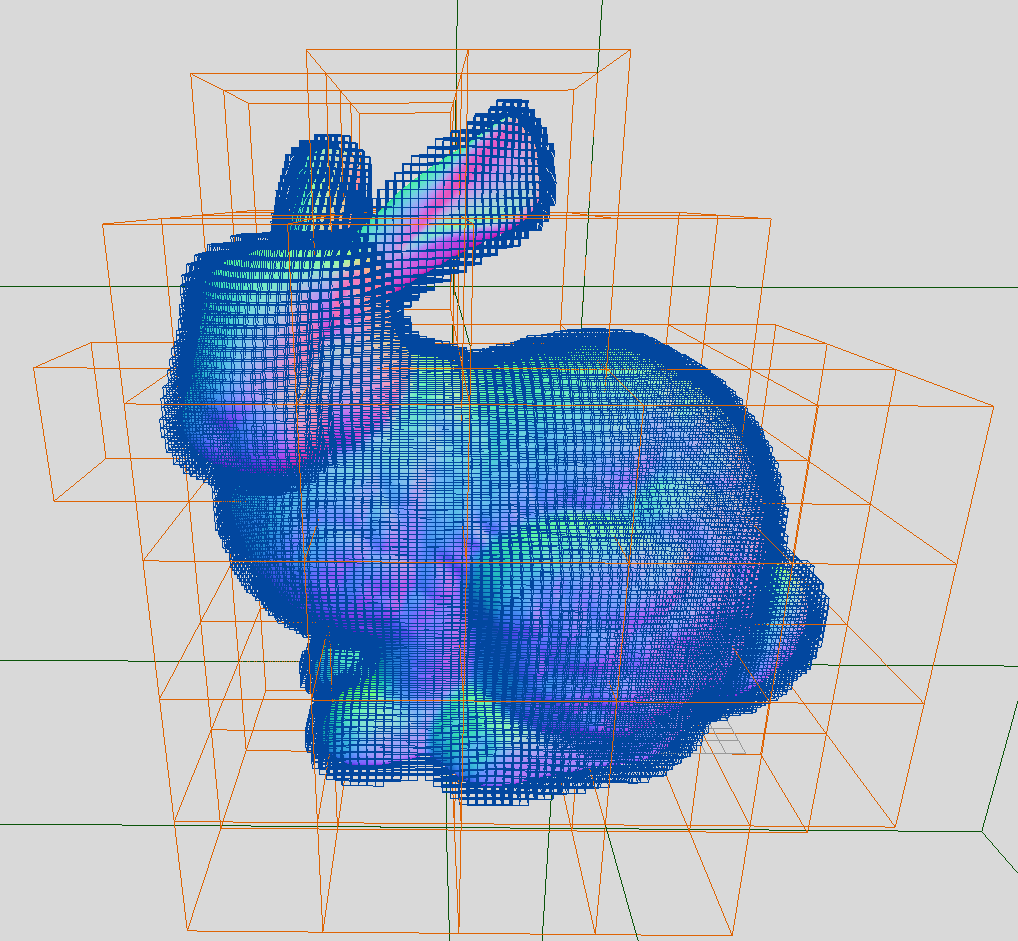
\includegraphics[width=0.5\textwidth]{figs/openvdb.PNG}}
   \caption{Narrow-band sparse grid and the extracted iso-surface from OpenVDB}
   \label{fig:narrow}
\end{figure}




We first make the following observation that helps us compute approximated ambient occlusion to the given iso-surface ~\citep{Evans:2006:FAG:1185657.1185834}. Given a point $p$ on the iso-surface and normalized outward normal direction $N$, we expect querying the narrow-band at point $p+iN$ will result into $i$ where $i$ is an integer i.e., stepping one unit along the normal should return a value of one. However, if there is some other object occluding $p$, this assumption does not hold since SDF hold the distance to the nearest object. 


Following this observation, we can estimate the ambient occlusion as 
$$
AO_{p} = exp(K \sum_{i=0}^{S}( SDF(p+iN) - i))
$$

for each $p$ point on the iso-surface mesh where $S$ is number of steps we take along the normal direction $N$,  $SDF()$ returns interpolated value of the signed distance field, and $K$ is a model-dependent constant. After obtaining the ambient occlusion constant, we multiply it by the vertex color. 



The above method is able to capture the affect of occluder that is far from the give point. Note that ambient occlusion usually done by integrating over a hemisphere by shooting many rays and compute the fraction of these rays that hits another object. The method above simplifies this process by integrating over a single line which may not be ideal. In particular, we noticed that this method can account for the occlusion effect from a far-away object. However, ambient occlusion should also account for the concavities of the surface. For that, we compute another ambient occlusion factor and blend it with the one above. The second ambient occlusion factor is computed as 
$$
AO_{p} = exp(-H*C)
$$

where $H$ is the mean curvature at $p$ and $C$ is a model dependent factor. 

We noticed that for some models, the effect of ambient occlusion is concentrated one a certain area where there is a large concavity. To smooth such effect, we applied a final step of Gaussian blur of the ambient occlusion factor. This works by changing the ambient occlusion at each vertex by the average of its neighbor vertices. 

\section{Results and Comparisons:}
In this section, we show some of the results we obtain of few models along with comparison with the ground-truth. The ground-truth is done following the outlines described above of shooting random rays from each mesh vertex implemented in~\citep{libigl}. 

Figure~\ref{fig:curv} shows the artifact of our method where most of the ambient occlusion factor is concentrated at concavities and thus need to be smoothed out.


\begin{figure}[!tbh]
\centering        
   \subfloat {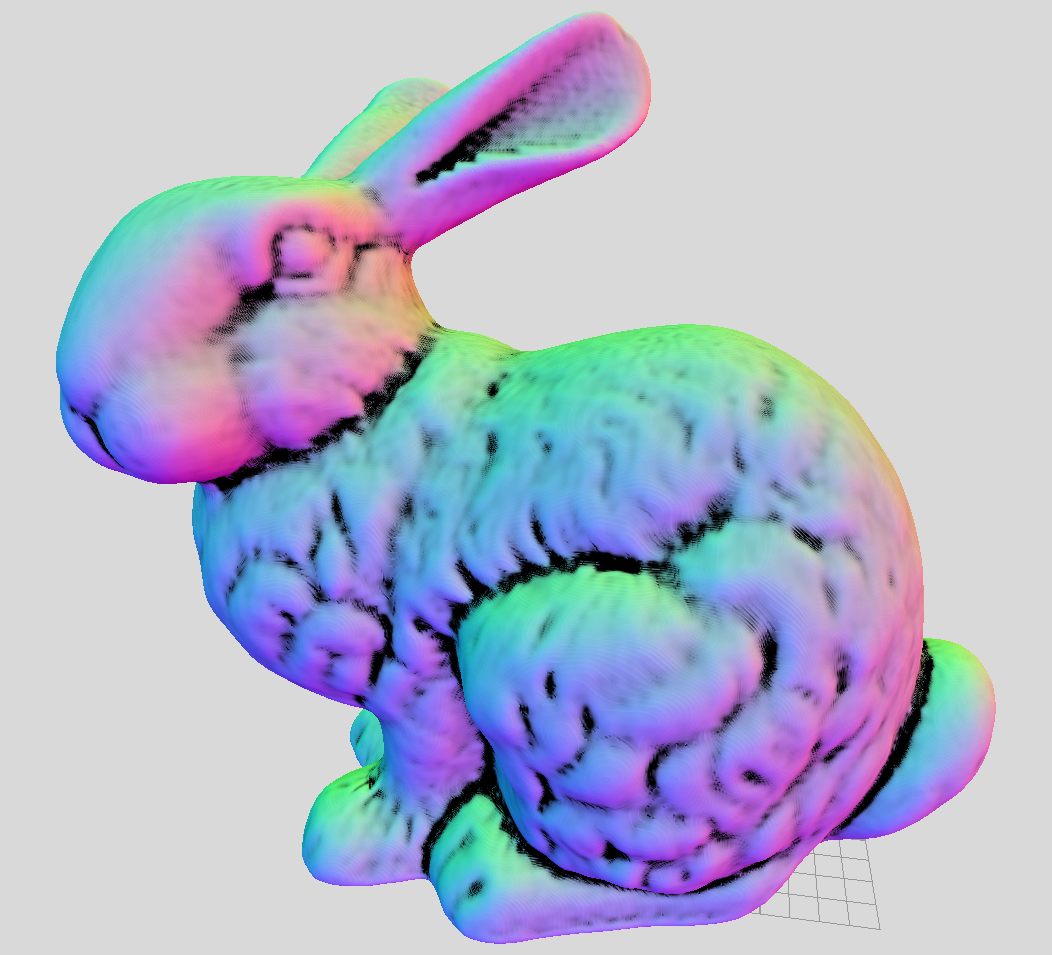
\includegraphics[width=0.4\textwidth]{figs/curvature.PNG}}
   \caption{Showing the artifact of our method where the ambient occlusion factor is concentrated in a certain regions}
   \label{fig:curv}
\end{figure}

\paragraph{Quality:} 

Figure~\ref{fig:bunny_ao} and Figure~\ref{fig:dragon_ao} show the impact of the ambient occlusion. We notice that after applying the ambient occlusion (bunny middle), the depth cue is improved and that adds more realism to the image. Comparing the results against the ground-truth, we find the we have capture most prominent area that should be occluded. Moreover, our results is less darkened overall where the occluded object is too far away (the Bunny back should be occluded by its ears). This is because we rely on the information in the narrow-band only.

\begin{figure}[!tbh]
\centering        
   \subfloat {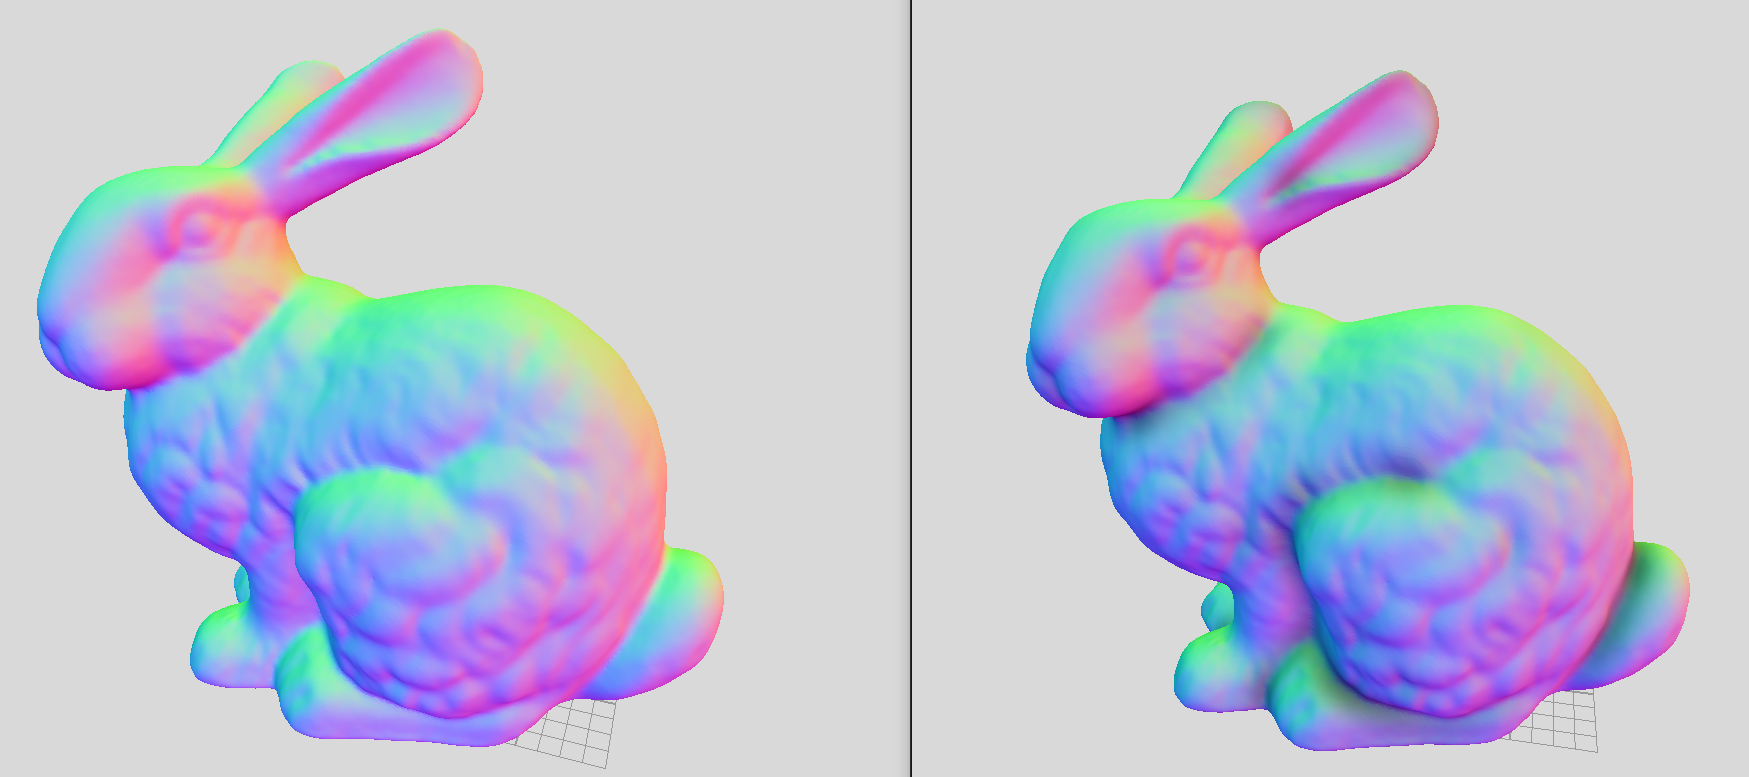
\includegraphics[width=0.7\textwidth]{figs/distance_only.PNG}}
   \subfloat {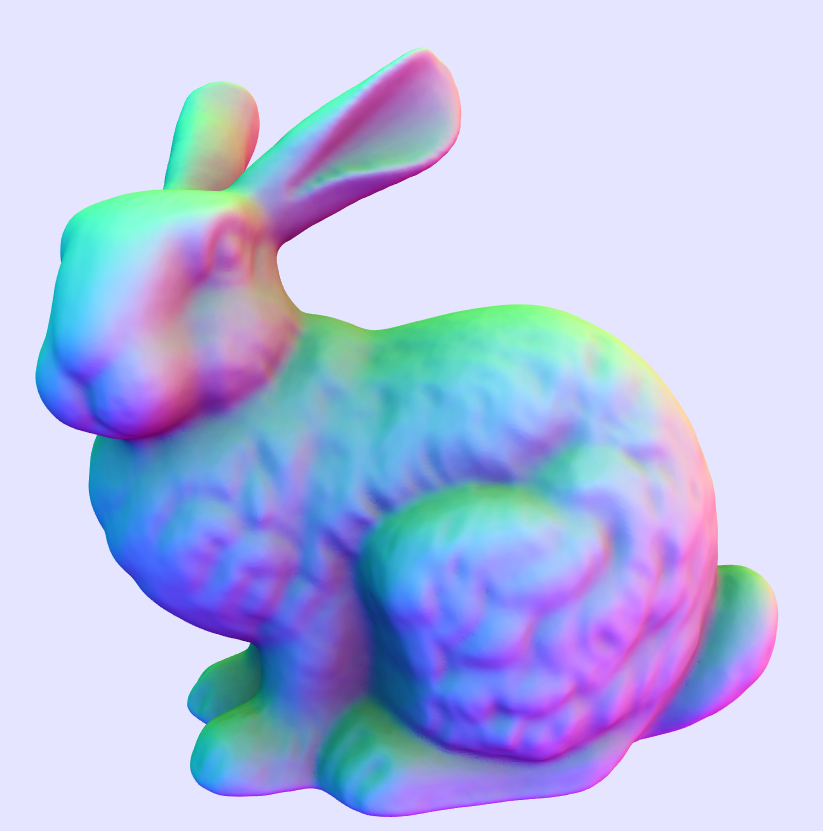
\includegraphics[width=0.308\textwidth]{figs/libigl_bunny.PNG}}
   \caption{Showing the impact of applying the ambient occlusion on a mesh of 1.5M vertices. Left is without ambient occlusion, middle is with ambient occlusion, right is the ground-truth}
   \label{fig:bunny_ao}
\end{figure}


\begin{figure}[!tbh]
\centering        
   \subfloat {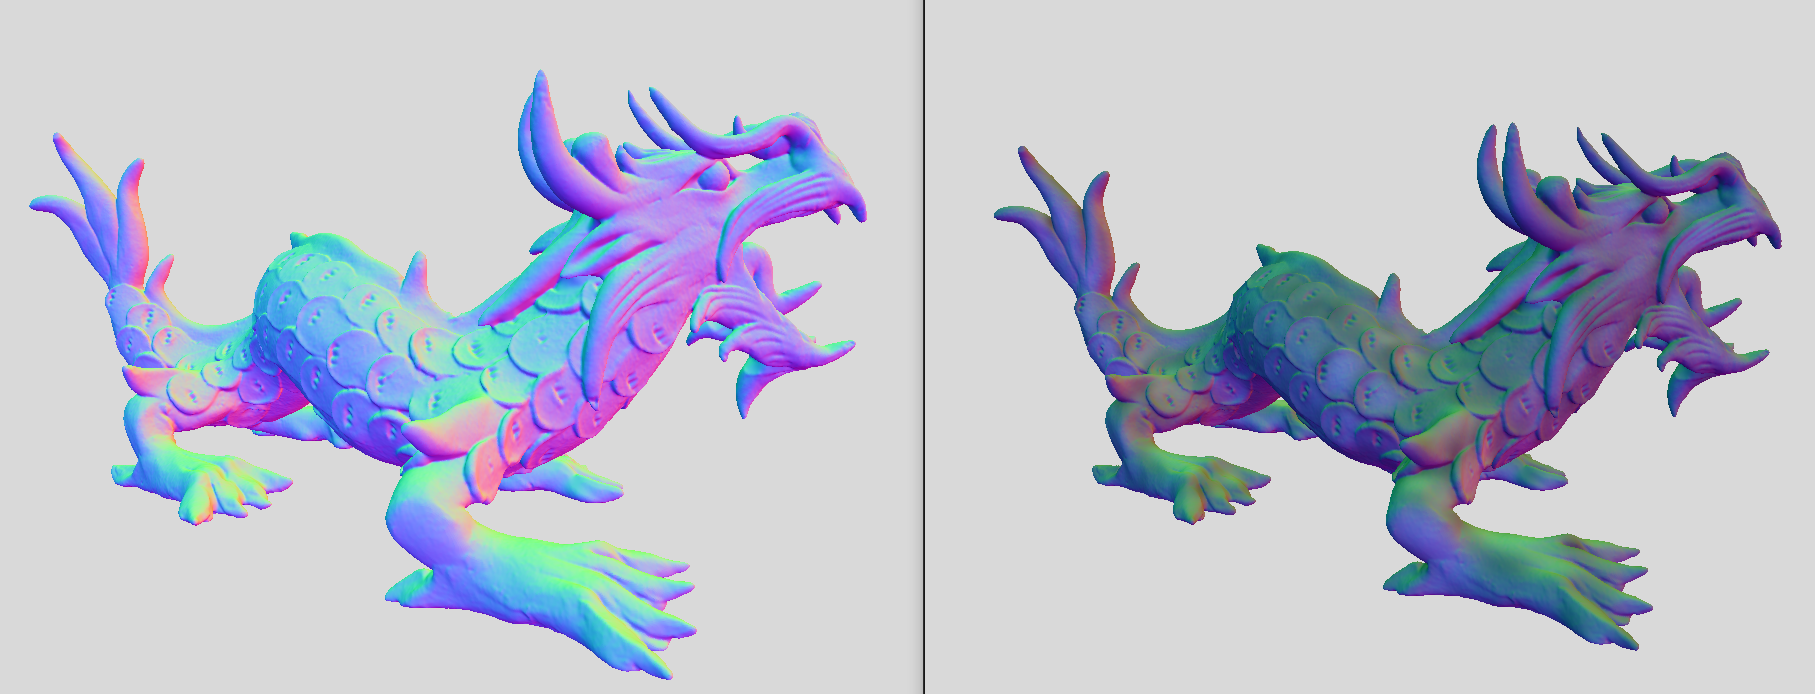
\includegraphics[width=0.65\textwidth]{figs/dragon.PNG}}
   \subfloat {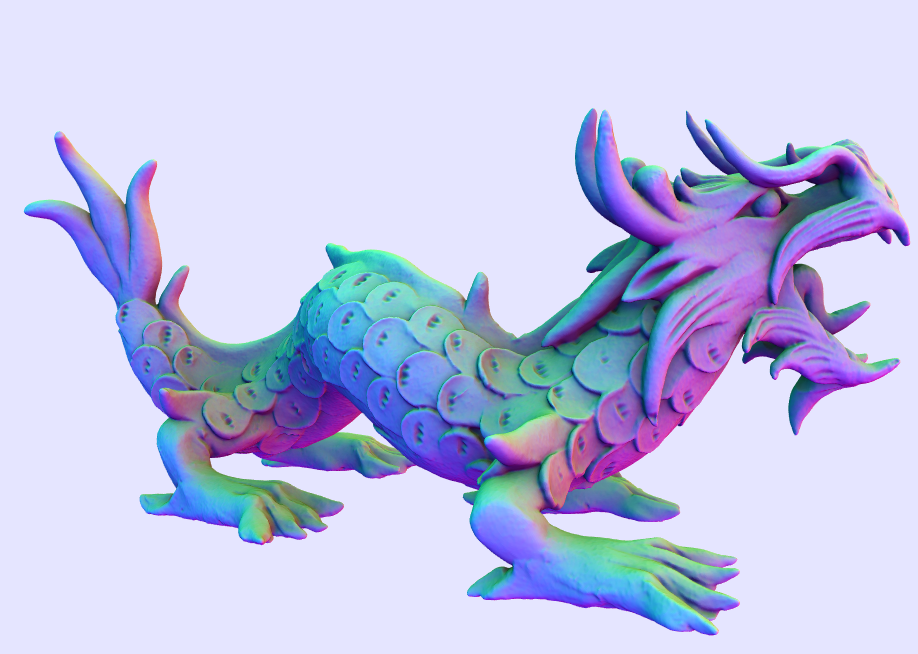
\includegraphics[width=0.35\textwidth]{figs/libigl_dragon.PNG}}
   \caption{Showing the impact of applying the ambient occlusion on a mesh of 3M vertices. Left is without ambient occlusion, middle is with ambient occlusion, right is the ground-truth}
   \label{fig:dragon_ao}
\end{figure}

\paragraph{Timing:}
For the Bunny model, we compare the timing it take for computing our ambient occlusion factor and compared it with the time of ray shooting. Ray shooting took 85 seconds ($\approx 1.5$ minute) which runs in parallel on 7 cores laptop. Our results only took $\approx 2$ seconds using only one thread which is $42X$ faster. This a significant speedup with very little lose in quality. We believe that this technique is more suitable for dynamic real-time applications. 


\section{Conclusion:}
In this project, we implemented a solution for ambient occlusion approximation for iso-surface visualization suitable for real-time dynamic situation. Our solution depends on having a narrow-band sparse grid around the extracted iso-surface which for some graphics and visualization applications is very efficient for the down-stream computation. Our solution is very fast compared compared to the ray-shooting method. As a future work, we would like to apply our technique on more models and compare against the screen-space ambient occlusion methods. Carrying out the computation in parallel in the vertex shader is another attractive direction for this technique. 
 
\medskip

\bibliography{mybib}


\end{document}
